\label{chapter: phase sep}

\section{Passive model B and Cahn-Hilliard dynamics}

\label{sec_PMB}

\subsection{The dynamical theory for conserved scalar order parameter} 

We have seen in~\autoref{chap_thermo} that the large-scale dynamics of systems that microscopically obey detailed balance minimize a free energy.
Therefore, model B that describes the dynamics of systems with a conserved scalar order parameters $\phi$ is generally written in terms of a functional ${\cal F}[\phi]$ that we express as
%
\begin{equation} \label{eq_F}
{\cal F}[\phi] = \intd{r} \left[ f(\phi) + \frac{\kappa(\phi)}{2}|\nabla\phi|^2\right],
\end{equation} 
%
where we have kept terms up to order $|\nabla \phi|^2$.
In Eq.~\eqref{eq_F} $f$, denotes the `bulk' free energy density and $\kappa(\phi) > 0$ is a generic function.
The bulk contribution consists of a free energy landscape due to e.g.\ entropic effects and interactions between microscopic elements, 
while the $\kappa$ term describes the cost of interfaces.

The dynamical equation for $\phi$ takes the general form
\begin{equation} \label{eq_phi}
\partial_t \phi(\bm r,t) = - \nabla \cdot \bm J(\phi) ,
\end{equation}
where the current $\bm J = \bm J_{\rm D} + \bm J_{\rm S}$ has a deterministic and stochastic contributions.
Up to some mobility $\bm M$, the deterministic part of the current $\bm J_{\rm D}$ is given by the chemical potential $\mu$:
\begin{equation} \label{eq_JD}
\bm J_{\rm D}(\phi) = - \bm M(\phi) \cdot \nabla \mu(\phi), \qquad \mu(\phi) = \frac{\delta {\cal F}}{\delta \phi} = f'(\phi) - \kappa(\phi) \nabla^2\phi - \frac{\kappa'(\phi)}{2}|\nabla\phi|^2 .
\end{equation}
The stochastic part, $\bm J_{\rm S}$, can be determined using the fluctuation dissipation relation:
\begin{equation} \label{eq_JS}
\bm J_{\rm S}(\bm r,t) = \sqrt{2 k_B T} \bm \sigma(\phi) \cdot \bm \Lambda(\bm r,t), \qquad \Lambda_i(\bm r,t)\Lambda_j(\bm r',t') = \delta_{ij}\delta^d(\bm r - \bm r')\delta(t - t'),
\end{equation}
with $\sigma_{ik}(\phi)\sigma_{jk}(\phi) = M_{ij}(\phi)$ (Einstein summation is implied).

\textit{{\bf Homework:}
Use the material presented in~\autoref{chap_thermo} to show that the choice~\eqref{eq_JS} ensures that the property of detailed balance is satisfied at the level of the dynamics of $\phi$.
Similarly to the Langevin equations satisfied by the particles degrees of freedom, Eq.~\eqref{eq_phi} is associated to a Fokker-Planck equation for the probability functional $\calP[\phi,t]$:
\begin{equation*}
\partial_t {\cal P}[\phi,t] = \intd{x} \frac{\delta}{\delta \phi}\left[ \nabla \cdot \left( {\cal P}[\phi,t] \bm J_{\rm D} - k_B T \bm M(\phi) \cdot \nabla \frac{\delta}{\delta \phi} {\cal P}[\phi,t]  \right) \right] .
\end{equation*}
Then, show that Eqs.~(\ref{eq_JD},\ref{eq_JS}) imply that the corresponding stationary distribution takes the Boltzmann form: ${\cal P}_{\rm s}[\phi] = \exp\left(-\tfrac{{\cal F}[\phi]}{k_B T} \right)$. 
}


The stochastic contribution to Eq.~\eqref{eq_phi} is usually written to study dynamical effects due to fluctuations (such as the roughening of interfaces, nucleation processes or to characterize the properties of the critical point...). Here, we will focus on the mean field properties of the models and thus drop the contribution from the noise ($\bm J_{\rm S} = \bm 0$).
Moreover, for simplicity we will restrict the presentation to the case of a scalar mobility $M(\phi) > 0$.

Although we keep the expression of the free energy density $f(\phi)$ general below,
its expression of course depends on the model of interest. 
Below, we describe two which are often considered: 
\begin{itemize}
\item {\bf The Flory-Huggins theory of polymer solutions.} Considering polymers in a solvent with respective volume fractions $\phi = v \rho$ and $\phi_{\rm sol} = v_{\rm sol} \rho_{\rm sol}$, 
the incompressibility of the solution implies that $\phi + \phi_{\rm sol} = 1$.
The Flory-Huggins free energy is then given by
$f_{\rm FH}(\phi) = k_B T \left[ \tfrac{1}{v} \phi \ln(\phi) + \tfrac{1}{v_{\rm sol}} (1-\phi)\ln(1-\phi) \right] + \chi \phi(1-\phi)$ where the first term accounts for the entropy contribution due to mixing of the polymer in the solvent, while the second term ($\propto \chi$) accounts for interactions. In the case where the latter are attractive, $\chi < 0$. For more details see e.g.~\cite{Eisele1990}. 
\item {\bf Cahn-Hilliard (Landau).} In general, the free energy can expanded in powers of $\phi$: $f_{\rm CH}(\phi) = \sum_i \tfrac{a_k}{k}\phi^k$ with the $\{a_k\}$ real coefficients allowed by the symmetries of the problem. 
Such expansion is generally considered as formally valid close to a critical point where $\phi$ is small (typically $\phi = (\rho - \rho_c)/\rho_c$ with $\rho_c$ the value of the density at the critical point) such that one usually truncates it at order $k = 4$.
Note that $f_{\rm CH}$ can be obtained from $f_{\rm FH}$ by expanding the logarithms.
\end{itemize}



\noindent {\it Spinodal decomposition} First, we investigate the condition for a homogeneous configuration with $\phi = \bphi$ to be stable to small perturbations.
Writing $\phi(\bm r,t) = \bphi + \delta \phi(\bm r,t)$, the perturbation $\delta \phi(\bm r,t)$ obeys from~\eqref{eq_phi} at linear order
\begin{equation} \label{eq_linear_phi}
\partial_t \delta \phi(\bm r,t) = \bar{M} \nabla^2 \left[ \left( \bar{f}'' - \bar{\kappa} \nabla^2\right)\delta \phi(\bm r,t)\right],
\end{equation}
where the bars stand for quantities evaluated at $\bphi$. 
Going into Fourier space, the growth rate associated to the mode with wavenumber $q$ is therefore $\lambda_q = -\bar{M} q^2(\bar{f}'' + \bar{\kappa} q^2)$.
As $\bar{M}$ and $\bar{\kappa}$ are both positive, the homogeneous configuration becomes unstable whenever $\bar{f}'' < 0$. 
This condition defines the so-called spinodal densities in the $(\bphi, k_B T$) phase diagram (Fig.~\ref{figeq}). 
In the region enclosed by the spinodals, any perturbation of homogeneous configurations grows exponentially fast, it is said that the system undergoes spinodal decomposition.

\textit{
{\bf Homework:}
Show that the emergence of phase-separation at equilibrium requires the presence of attractive interactions.
Hint: you can show this by considering the free energy ${\cal F}[\phi] = k_B T\intd{r} \phi (\ln(\phi) - 1) + \intd{r} \chi \phi^2(\bm r)$.
Propose an interpretation for the two integrals contributing to $\cal F$.
}

%%%%%%%%%%%%%%%%%%%%%%%%%%%%
\begin{figure}[b!]
	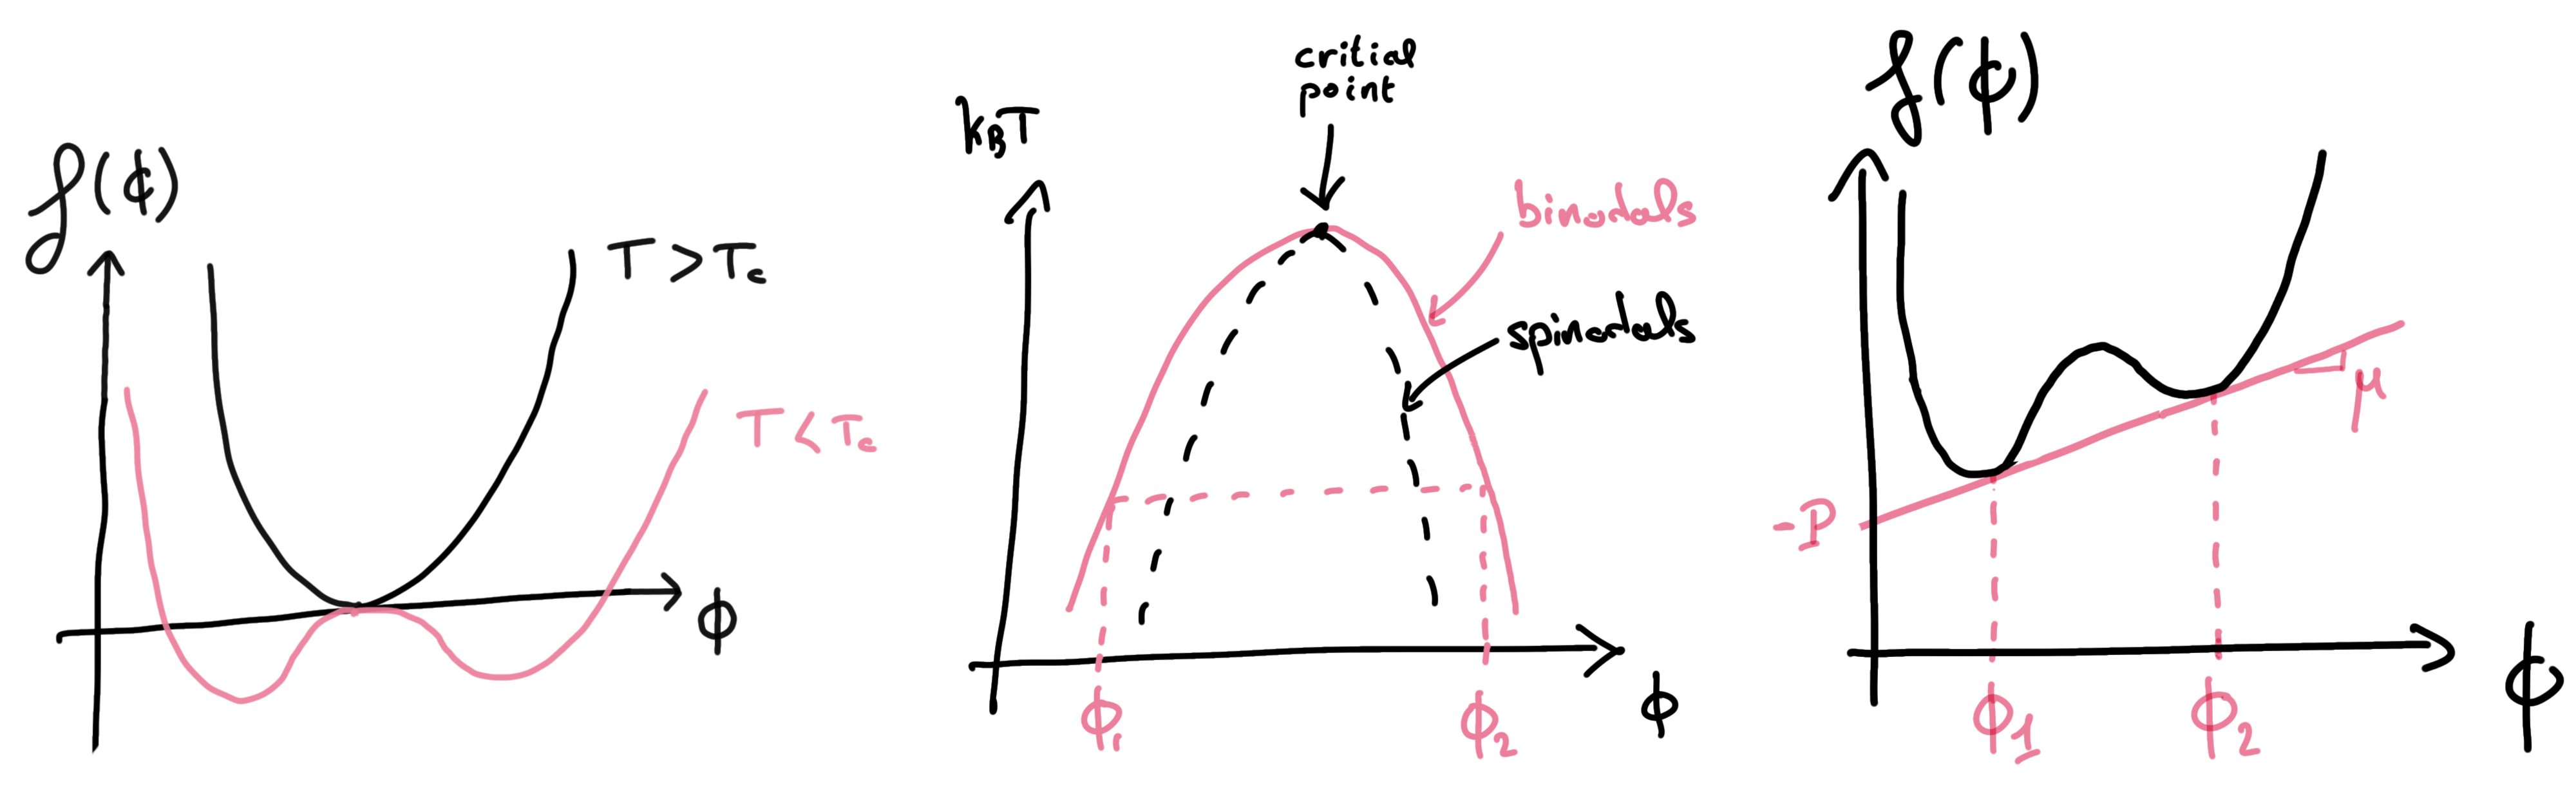
\includegraphics[width=\textwidth]{Figures/equilibrium_ps.pdf}
	\caption{Left: Typical Landau free energy landscapes above and below the critical point. 
	Center: phase diagram in the plane spanned by density and temperature showing the spinodals, binodals, and the critical point. 
	Right: Common tangent construction allowing to determine the coexistence densities in the phase separated regime.}
	\label{figeq}
\end{figure}
%%%%%%%%%%%%%%%%%%%%%%%%%%%%

\noindent {\it Binodal densities and the composition of phase separated configurations} 
The linear stability analysis does not tell us much about the state of the system long after the instability arises.
After the system undergoes spinodal decomposition, it goes through a coarsening regime until it phase separates into coexisting domains of different volumes and densities.
To determine the coexisting densities, we use the conservations of the total volume ${\cal V}$ and of the field $\phi$. 
We moreover work in the thermodynamic limit ${\cal V} \to \infty$ such that contributions from the interfaces can be safely neglected and we only consider the bulk contribution $f(\phi)$.
In a stationary phase-separated regime where the system is partitioned into two domains with $\phi = \phi_{1,2}$ and of respective volumes ${\cal V}_{1,2}$, 
the free energy~\eqref{eq_F} takes the trivial form
\begin{equation} \label{eq_F_ps}
{\cal F} = f(\phi_1) {\cal V}_1 + f(\phi_2) {\cal V}_2.
\end{equation} 
Denoting the mean value of $\phi$ as $\bphi$, the conservations of the total mass and volume impose
\begin{equation} \label{eq_constraints_binodals}
\phi_1 {\cal V}_1 + \phi_2 {\cal V}_2 = \bphi {\cal V}, \qquad  {\cal V}_1 + {\cal V}_2 = {\cal V} .
\end{equation} 
To determine the values $\phi_1$ and $\phi_2$, we minimize the free energy~\eqref{eq_F_ps} imposing~\eqref{eq_constraints_binodals}.
This is done by adding Lagrange multipliers ($\mu,P$) to ${\cal F}$, such that we define $\tilde{\cal F} = {\cal F} + P({\cal V}_1 + {\cal V}_2) - \mu(\phi_1 {\cal V}_1 + \phi_2 {\cal V}_2)$.
Minimizing $\tilde{\cal F}$ wrt the values of density and volume of each of the two phases, we get
\begin{align} \label{eq_binodal_mu}
\frac{\partial \tilde{\cal F}}{\partial \phi_i}  & = {\cal V}_i (f'(\phi_i) - \mu) = 0 , \\
\label{eq_binodal_P}
\frac{\partial \tilde{\cal F}}{\partial {\cal V}_i}  & = f(\phi_i) - \mu \phi_i + P = 0 ,
\end{align}
with $i = 1,2$.
Eq.~\eqref{eq_binodal_mu} imposes that the chemical potential $\mu = f'(\phi_1) = f'(\phi_2)$ takes identical values in both phases (\emph{diffusive equilibrium}),
while Eq.~\eqref{eq_binodal_P} ensures the equality of pressures (\emph{mechanical equilibrium}).
Therefore, one can determine graphically the values of $\phi_1$ and $\phi_2$ from a common tangent construction 
on the free energy landscape. 
Indeed, the equality of chemical potentials imposes equal slopes of $f$ at $\phi_1$ and $\phi_2$, 
while equality of pressures imposes a common intercept on the vertical axis as shown in Fig.~\ref{figeq}

Varying, e.g.\, the system temperature, the coexistence values $\phi_{1,2}$ define the \emph{binodal curves},
and meet the spinodals we determined previously at the critical point. 
As shown in Fig.~\ref{figeq}, the spinodals and binodals generally do not coincide, such that there are regions of the phase diagram 
where phase separated configurations exist (and are stable) but the homogeneous state at $\phi = \bphi$ is also linearly stable.
In practice, if we now put back noise into the picture in these regions the homogeneous state will typically disappear 
not through the deterministic growth of an infinitesimal perturbation, 
but because of stochastic nucleation events which correspond to large perturbations and are thus captured by the linear stability analysis.
Within the binodal region, the system thus always phase separates over long times into two distinct domains 
where $\phi$ takes values $\phi_{1,2}$ and whose volumes linearly interpolate between 0 and ${\cal V}$ for $\bphi \in [\phi_1;\phi_2]$ due to the condition~\eqref{eq_constraints_binodals}, 
namely
\begin{equation}
{\cal V}_1 = \frac{\phi_2 - \bphi}{\phi_2 - \phi_1} {\cal V}, \qquad {\cal V}_2 = {\cal V} - {\cal V}_1 = \frac{\bphi - \phi_1}{\phi_2 - \phi_1} {\cal V},
\end{equation} 
which is known as the \emph{lever rule}.\\

\noindent {\it The coarsening dynamics} So far, we have discussed the linear instability of homogeneous solutions and the relative composition of phase-separated states.
Of course, another interesting aspect of phase separation concerns how one moves from one to the other. 
Without entering into details (a relevant review paper on the topic is~\cite{Bray1994}), 
the coarsening process leading to phase separation can be understood by taking into account finite size effects, 
i.e.\ by considering the nonlocal contributions to the free energy which we have neglected above.
Doing this, one finds that the pressure inside a spherical droplet increases with its interface curvature, 
leading to a diffusive flux from small to large droplets. 
Over long times, small droplets thus typically shrink at the expense of larger ones, which is known as \emph{Ostwald ripening}.
One can moreover show that under this process the mean droplet radius grows in a universal manner as $\sim t^{1/3}$,
so that the asymptotic ($t \to \infty$) state inevitably consists of two macroscopic phase separated domains. 






















